\section{Framebuffer DMA processor}
\label{sec:framebuffer_dma}

A framebuffer is a portion of memory which holds the current frame, allowing the hardware blocks either side to act in complete isolation. Both sides of the link use framebuffers, though their purpose differs. On the receiver side the framebuffer stores each frame before it is written to flash storage. Firmware inside the Zynq \gls{ps} \marginpar{Explain the Zynq PS} can draw to the frame in real-time, adding helpful indicators such as the currently connected sensor module and gridlines to aid the photographer's composition process. On the transmitter side the framebuffer serves a different purpose. A critical flaw in the design of the \gls{dvi} receiver causes the link to break if the incoming pixel clock is less than \SI{40}{\mega\hertz} --- a potential issue because the OV7670's pixel clock is only \SI{12}{\mega\hertz}. To mitigate this, the transmitter sends out duplicate frames, thus bringing the pixel clock up into the region required for correct operation.

The space required to store frames is a direct function of the image resolution. As the OV7670 outputs frames in 640 x 480 resolution, a \SI{307.2}{\kilo\byte} framebuffer is required. While \glspl{fpga} usually contain a small amount of internal block RAM, there is insufficient space for storing an entire frame. Though its access is significantly more complicated, the Zynq-7000 includes a hard DDR controller which can be utilised to store the frames in external DDR3 memory instead --- the Zybo development board contains \SI{512}{\mega\byte} of RAM, which is more than sufficient for storing a single frame.

\marginpar{Diagram of internal Zynq arch - access to DDR}

\subsection{AXI}
Due to the internal architecture of the Zynq-7000, external RAM is only accessible from the \gls{ps}, thus incoming frames which are processed by the \gls{pl} must be fed into the \gls{ps} before they can be stored in the RAM. Fortunately the \gls{pl} and \gls{ps} are able to exchange data using the \gls{axi} interface, which was designed to provide a single interconnect for IP across all domains. While there are several different variants of \gls{axi} (a comparison of which is found in Table \ref{table:axi_comparison}), they all operate in fundamentally the same way. \gls{axi} is used to connect a master device to a slave device using one or more channels which are used to carry out transactions. A standard AXI4 connection will consist of five channels:
\begin{itemize}
  \item Read Address Channel
  \item Write Address Channel
  \item Read Data Channel
  \item Write Data Channel
  \item Write Response Channel
\end{itemize}
(http://www.xilinx.com/support/documentation/ip_documentation/axi_ref_guide/latest/ug1037-vivado-axi-reference-guide.pdf)

\begin{table}[]
\centering
\caption{Comparison of AXI interfaces. Adapted from (http://www.xilinx.com/support/documentation/ip_documentation/axi_ref_guide/latest/ug1037-vivado-axi-reference-guide.pdf).}
\label{table:axi_comparison}
\begin{tabular}{llll}
              & AXI4                               & AXI4-Lite                      & AXI4-Stream                \\
Dedicated for & High-performance and memory-mapped & Register-style interfaces      & Non-address based IP       \\
Burst         & Up to 256                          & 1                              & Unlimited                  \\
Data width    & 32 - 1024 bits                     & 32 / 64 bits                   & Anything                   \\
Applications  & Embedded, memory                   & Small footprint logic, control & DSP, video, communications
\end{tabular}
\end{table}

As separate channels are used for reading and writing, device communication is fully bi-directional. In addition to the address and data signals, extra signals are provided for control and synchronisation to ensure that a device can only begin a transaction when the other device is ready. Figure \ref{fig:axi_architecture} illustrates a typical AXI4 interface. 

\begin{figure}
\centering
\begin{subfigure}{.5\textwidth}
  \centering
  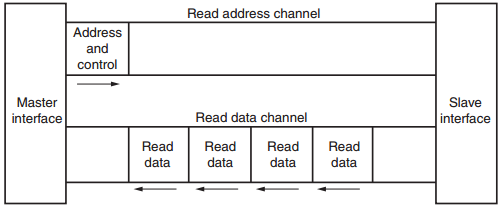
\includegraphics[width=.4\linewidth]{./img/axi_read.png}
  \caption{Read Channel}
\end{subfigure}%
\begin{subfigure}{.5\textwidth}
  \centering
  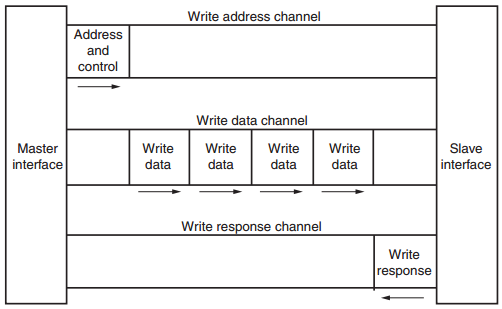
\includegraphics[width=.4\linewidth]{./img/axi_write.png}
  \caption{Write Channel}
\end{subfigure}
\caption{Architecture of AXI4 Read and Write Channels. (http://www.xilinx.com/support/documentation/ip_documentation/axi_ref_guide/latest/ug1037-vivado-axi-reference-guide.pdf)}
\label{fig:axi_architecture}
\end{figure}

All hardware inside the Zynq can be addressed from the \gls{ps} provided it has been connected via \gls{axi}. AXI requires all devices to be assigned an address which complies with the address map in Table \ref{table:zynq_address_map}. For example, the \gls{axi} master port \texttt{M\_AXI\_GP0} on the \gls{ps} has the address range \texttt{0x4000_0000} to \texttt{0x7FFF_FFFF}. Any \gls{axi} slave devices in the \gls{pl} assigned an address in this range can be accessed from the \gls{ps}. Conversely, any \gls{axi} master devices in the \gls{pl} connected to the \gls{ps} slave port \texttt{S\_AXI\_HP0} can access most of the DDR address range.

\begin{table}[]
\centering
\caption{Zynq-7000 system-level address map. (http://www.xilinx.com/support/documentation/user_guides/ug585-Zynq-7000-TRM.pdf)}
\label{table:zynq_address_map}
\begin{tabular}{lllll}
Address range                             & CPUs and ACP & AXI\_HP & Other bus masters & Notes                                                 \\
\multirow{4}{*}{0000\_0000 to 0003\_FFFF} & OCM          & OCM     & OCM               & Address not filtered by SCU and OCM is mapped low     \\
                                          & DDR          & OCM     & OCM               & Address filtered by SCU and OCM is mapped low         \\
                                          & DDR          &         &                   & Address filtered by SCU and OCM is not mapped low     \\
                                          &              &         &                   & Address not filtered by SCU and OCM is not mapped low \\
\multirow{2}{*}{0004\_0000 to 0007\_FFFF} & DDR          &         &                   & Address filtered by SCU                               \\
                                          &              &         &                   & Address not filtered by SCU                           \\
\multirow{2}{*}{0008\_0000 to 000F\_FFFF} & DDR          & DDR     & DDR               & Address filtered by SCU                               \\
                                          &              & DDR     & DDR               & Address not filtered by SCU                           \\
0010\_0000 to 3FFF\_FFFF                  & DDR          & DDR     & DDR               & Accessible to all interconnect masters                \\
4000\_0000 to 7FFF\_FFFF                  & PL           &         & PL                & General Purpose Port \#0 to the PL, M\_AXI\_GP0       \\
8000\_0000 to BFFF\_FFFF                  & PL           &         & PL                & General Purpose Port \#1 to the PL, M\_AXI\_GP1       \\
E000\_0000 to E02F\_FFFF                  & IOP          &         & IOP               & I/O Peripheral registers                              \\
E100\_0000 to E5FF\_FFFF                  & SMC          &         & SMC               & SMC Memories                                          \\
F800\_0000 to F800\_0BFF                  & SLCR         &         & SLCR              & SLCR registers                                        \\
F800\_1000 to F880\_FFFF                  & PS           &         & PS                & PS System registers                                   \\
F890\_0000 to F8F0\_2FFF                  & CPU          &         &                   & CPU Private registers                                 \\
FC00\_0000 to FDFF\_FFFF                  & Quad-SPI     &         & Quad-SPI          & Quad-SPI linear address for linear mode               \\
\multirow{2}{*}{FFFC\_0000 to FFFF\_FFFF} & OCM          & OCM     & OCM               & OCM is mapped high                                    \\
                                          &              &         &                   & OCM is not mapped high                               
\end{tabular}
\end{table}

\marginpar{Include address map of actual design}

\subsection{Linebuffers}
Due to the high complexity of the DDR controller, memory operations are not instantaneous and have non-deterministic latencies, thus an additional buffer must be placed between the incoming frames from the \texttt{ov7670\_capture} block and framebuffer, and a second between the framebuffer and the \texttt{rgb2dvi} module.

Each line of the input frame is written into a \SI{2048}{\kilo\bit} linebuffer pixel-by-pixel. 

During the blanking period an interrupt on the \gls{ps} is triggered 

\subsection{\texttt{i\_buf\_controller} module}

The \texttt{i_buf_controller} module is a simple shim which writes each line of the video into the linebuffer and triggers interrupts on the \gls{ps} to initiate a \gls{dma} transfer into the DDR framebuffer. Upon detecting the \texttt{vde} signal going high, the input buffer controller starts writing each incoming pixel into the linebuffer. The block RAM can either be configured in standalone mode or for use with an AXI BRAM Controller instance. The block RAM has its own address space (starting at \texttt{0x0000} up to however large the block RAM is), and so an AXI BRAM Controller instance is placed between the block RAM and input AXI CDMA instance (\texttt{i\_axi\_cdma}) to translate between the two address spaces.

As the block RAM is operating in BRAM Controller mode the following Block Memory Generator configuration is used:
\begin{itemize}
  \item 32-bit data width
  \item 2048-bit data depth
  \item 32-bit address width
  \item Byte addressing

\subsection{AXI CDMA and buffer control firmware}


\marginpar{Diagram of OV7670 -> framebuffer -> DVI isolation, and DVI -> framebuffer -> SD / screen}